\lecture{1}{Tue 14 Jan 2020 14:30}{393 Lab 1}

%\section{Introduction}
%In today's lab we learned about the basics of Simulink and controlling our simple motor through MatLab. 

\section{Deliverables}

\subsection{Plots}

\begin{figure}[H]
	\centering
	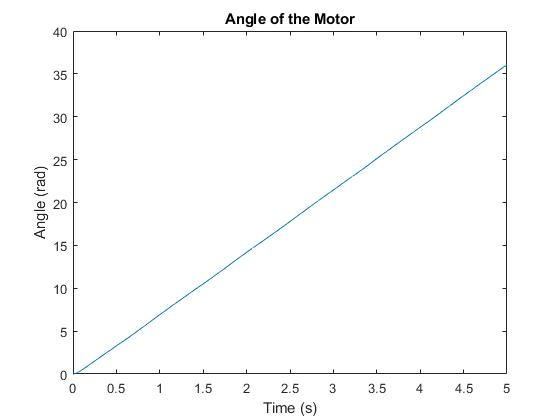
\includegraphics[width=0.8\textwidth]{./figures/theta_plot.jpg}
	\caption{Plot of current angle of the motor}
	\label{fig:theta_plot}
\end{figure}
\begin{figure}[H]
	\centering
	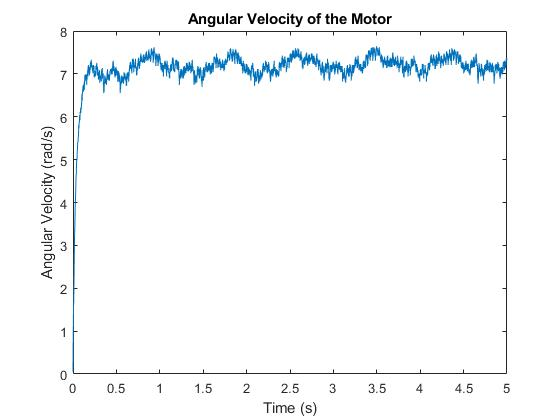
\includegraphics[width=0.8\textwidth]{./figures/omega_plot.jpg}
	\caption{Plot of the angular velocity of the motor}
	\label{fig:omega_plot}
\end{figure}
\subsection{Steady State Angular Velocity}

We found the steady state angular velocity $K_{E}\tau $ to be equal to $7.23 \text{ rad}/s$  by averaging the value of omega over half the duration, once the experiment hit steady state. 

\begin{verbatim}
    kEtau = mean(omega.signals.values(1250:2501));
\end{verbatim}

The slope of the encoder plot for $\omega$ was approximately $7.2$, which matches our calculated value. 
\subsection{Motor Constant}

The motor constant $\tau $ of the motor was found to be $0.0360 \text{ s}$ by using MatLab, finding the time at which $\omega$ at $\tau $.
\begin{verbatim}
    e = exp(1);
    omega_at_tau = kEtau * (1 - exp(-1));
    i = 1;
    while omega.signals.values(i) < omega_at_tau
        i = i + 1;  
    end
    tau = omega.time(i)	
\end{verbatim}
Plot at $t = \tau $:
\begin{figure}[H]
	\centering
	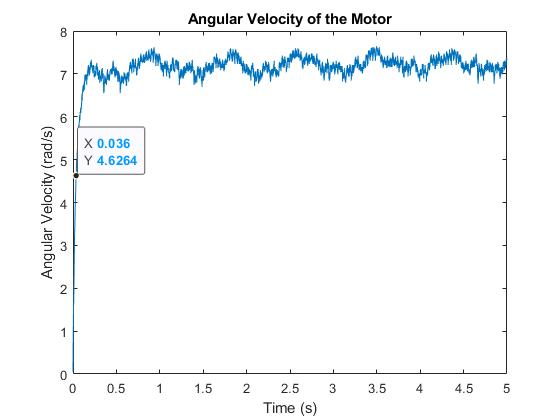
\includegraphics[width=0.8\textwidth]{./figures/omega_plot_at_tau.jpg}
	\caption{Plot of angular velocity with $\tau $ marked}
	\label{fig:omega_plot_at_tau}
\end{figure}

\subsection{Motor Torque Constant}
The motor torque constant $K_{E}$ was found to be $201.03 \text{ rad}/s^2$, via:
\begin{verbatim}
        kE = kEtau / tau
\end{verbatim}
